\documentclass{scrartcl}
\usepackage[utf8]{inputenc}
\usepackage{graphicx}
\usepackage{subfigure}
\usepackage{supertabular}
\usepackage{float}
\usepackage{booktabs, tabularx}
\begin{document}

\title{Short documentation for the RAxML Workbench}
\maketitle
\tableofcontents
\section{Panel nesting overview}
	\begin{figure}[htb]
		\centering
		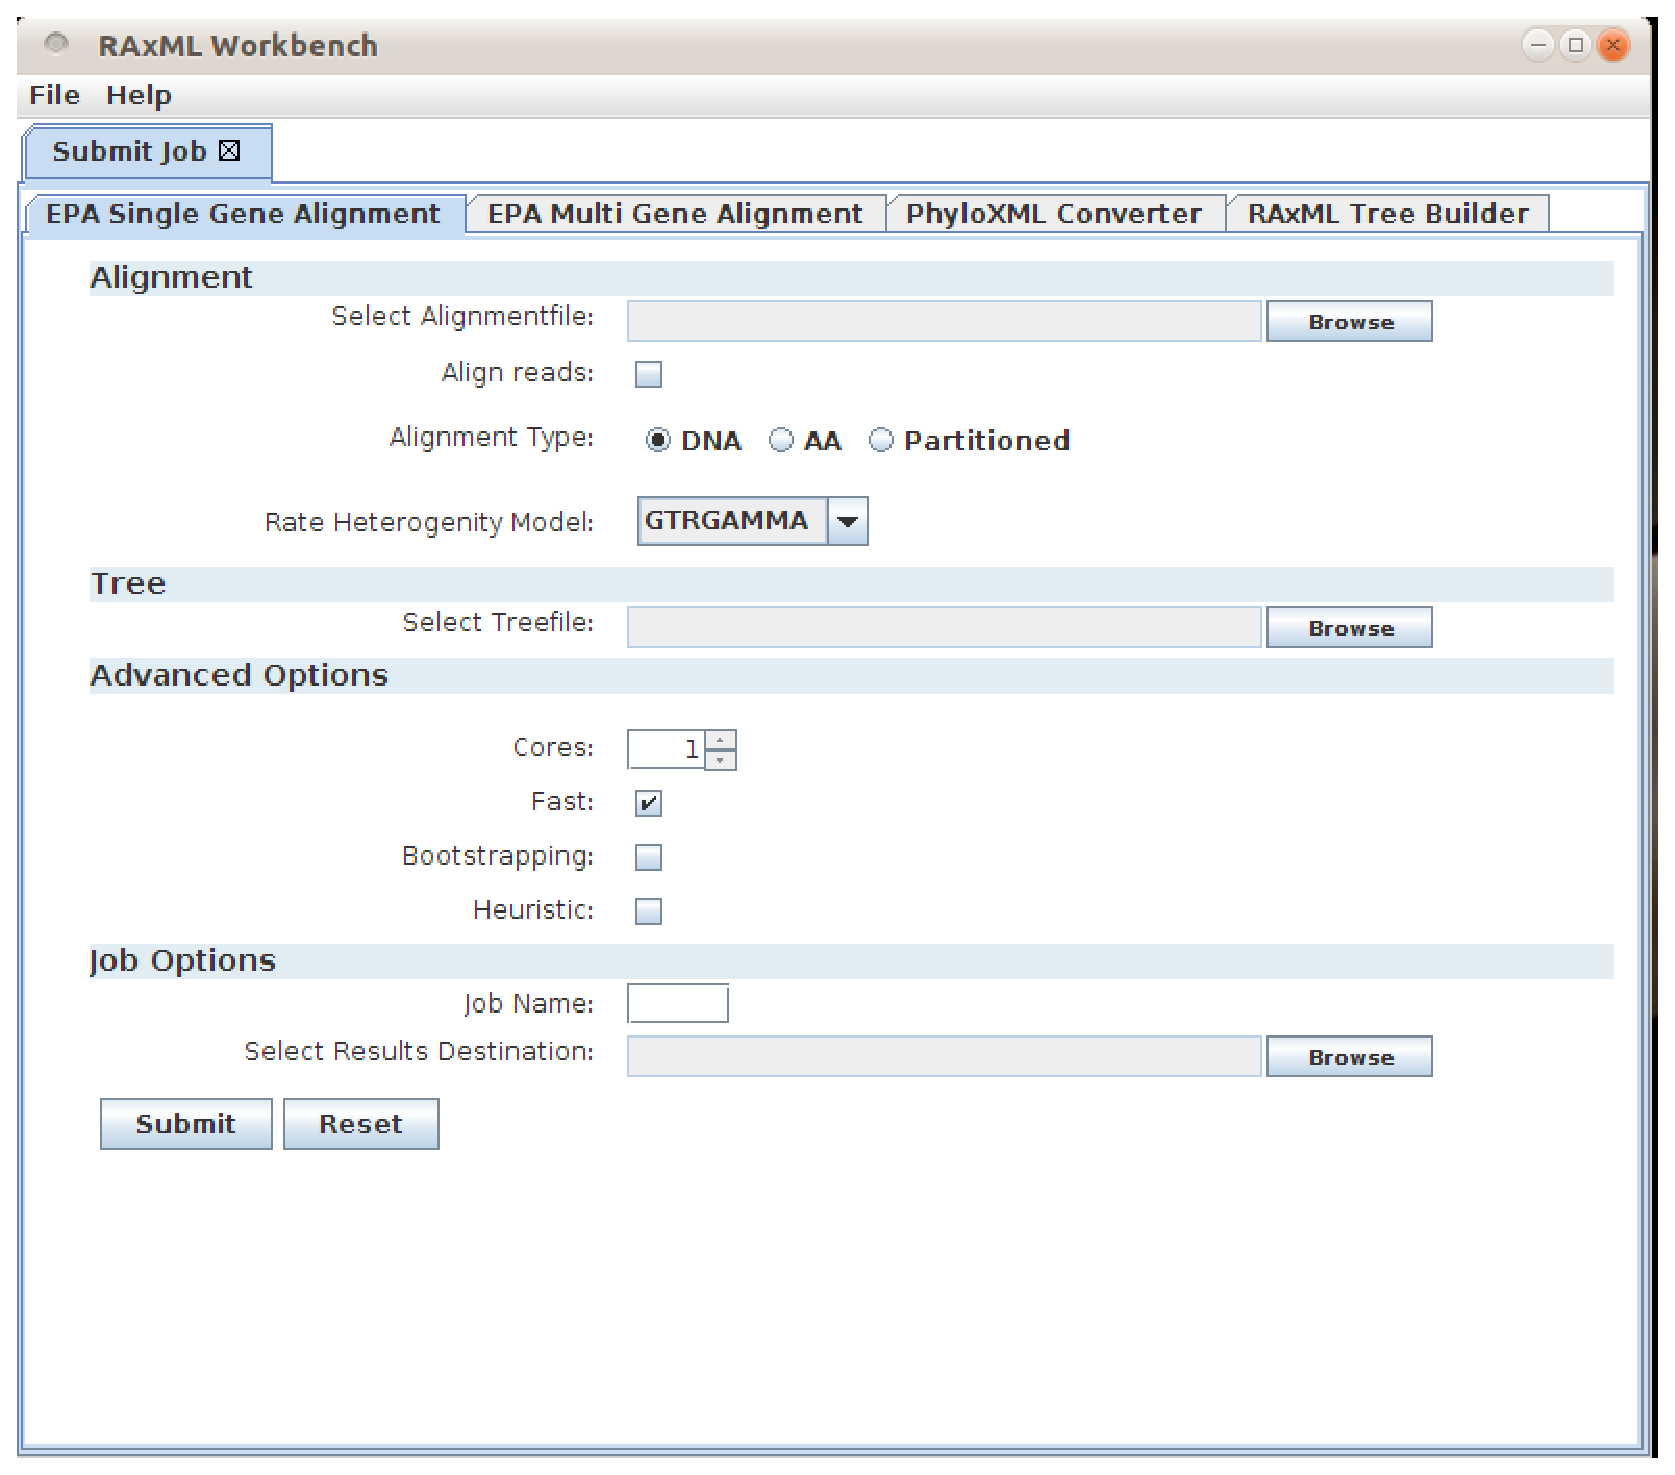
\includegraphics[scale=0.40]{./workbench_complete}
		\caption{The start-up presentation of the GUI}
		\label{fig:wbcomplete}
	\end{figure}
\noindent	The GUI in figure \ref{fig:wbcomplete} consists basically of three layers. The first layer is the MainFrame. It holds the menu bar at the top and a penal called \textit{WorkflowPanel} beneath it that administrates all jobs of the user in a TabbedPane. The second layer consists of \textit{Job} objects that can be added and removed from the Workflow's TabbedPane. These Job objects are panels themselves and can be a TabbedPane again, holding the different submission panels, a \textit{WaitingPanel} or a \textit{ResultsPanel}. The last layer are the different submission panels (\textit{SgaFormPanel, MgaFormPanel, PhyloXMLConverterFormPanel and TreeBuilderFormPanel}) which represent the input forms for the submissions, the WaitingPanel that is shown when a job is running,  and the ResultsPanel which shows the output files and provides an interface to the treeviewer. 

\section{The MainFrame}
	\begin{figure}[htb]
		\centering
		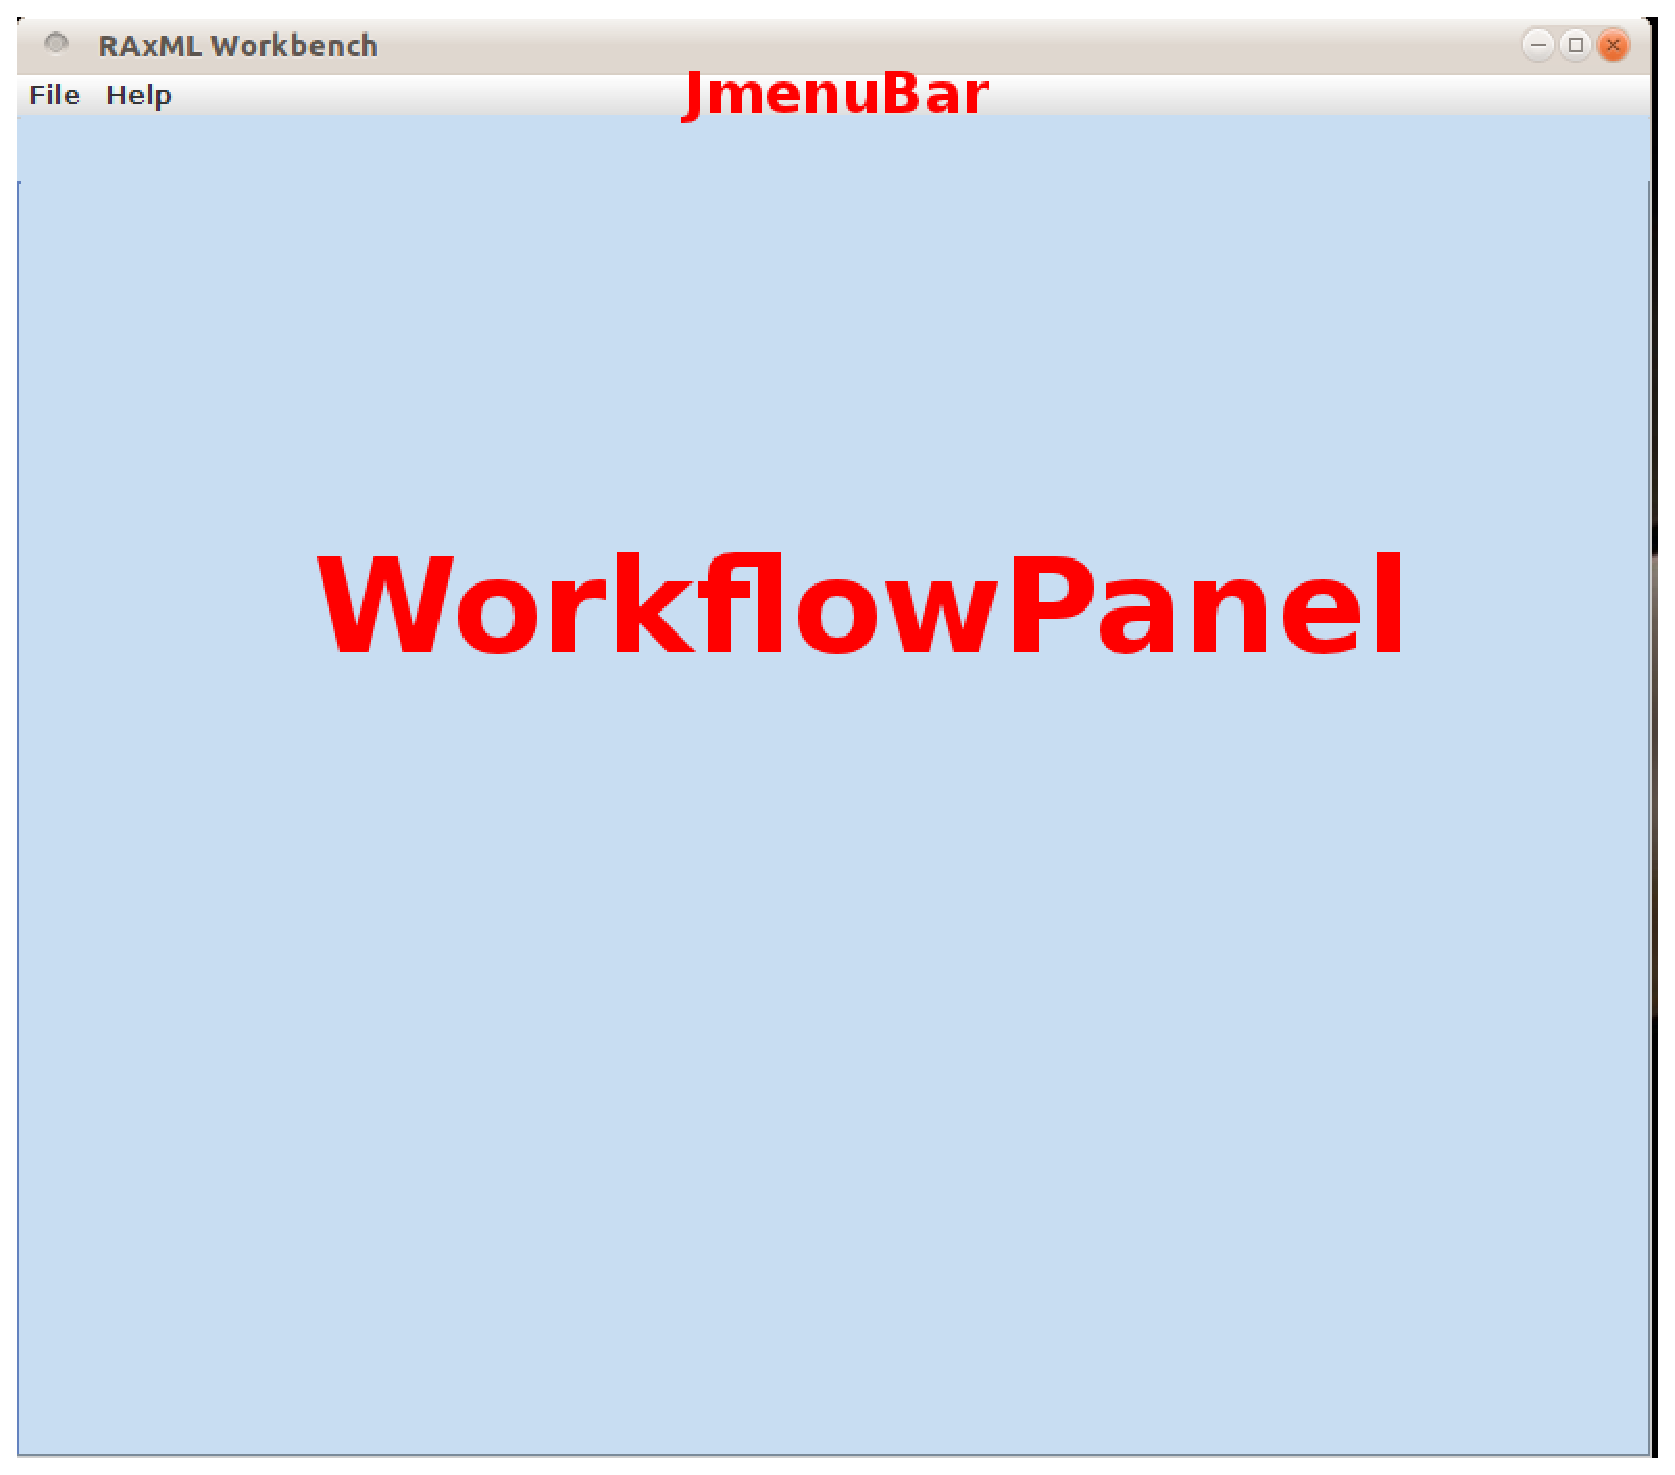
\includegraphics[scale=0.2]{./MainFrame}
		\caption{The MainFrame}
		\label{fig:mainframe}
	\end{figure}
\noindent	As mentioned before, the MainFrame panel (figure \ref{fig:mainframe}) holds  a JMenuBar which is shown on the top of the GUI and a WorkflowPanel at the bottom which contains a TabbedPane that holds the Job objects. The actions of the JMenuBar are also controlled in this Panel, like showing the help pdf or exiting the application for example.


\section{The WorkflowPanel}
	\begin{figure}[htb]
		\centering
		
\includegraphics[scale=0.2]{./workFlowPanel}
		\caption{The WorkflowPanel}
		\label{fig:wf}
	\end{figure}
\noindent	The WorkflowPanel (figure \ref{fig:wf}) administrates the different Job panels stored in its TabbedPane. Jobs can be removed or added.  
	
\section{The Job (Panel)}

	\begin{figure}[htb]
		\centering
		\includegraphics[scale=0.25]{./Job}
		\caption{The Job(Panel), the Job panel holds different panels within the submission process. From left to right: At the left, a new Job is opened and the different submission forms are shown. After the submission, the Job changes its content to a WaitingPanel (middle). After the submission has been processed and finished it changes its content again to a ResultsPanel (right).}
		\label{fig:job}
	\end{figure}
\noindent	This panel provides the different user interfaces available within the GUI. During a submission process, the Job object changes its content multiple times as can be seen in figure \ref{fig:job}. 
	\section{The Submission Panels}
		\subsection{SgaFormPanel}
			This panel contains the complete input form for the EPA single gene submission similar to the EPA  webserver one. The inputs are validated and redirected to the Submission object which performs the submission. 
		\subsection{MgaFormPanel}
			This panel contains the complete input form for the EPA multi gene submission similar to the EPA webserver one
		\subsection{PhyloXMLConverterFormPanel}
			The PhyloXMLConverterFormPanel provides an user interface for converting classification and treefiles into a phyloXML file that can be read by the treeviewer. It directly calls the convertToPhyloXML java program and performs the submission. 
		\subsection{TreebuilderFormPanel}
			This allows the user to have a simplified access to the RAxML treebuilder.  It performs the submission through the Submission class. 
	\section{WaitingPanel}
		The Waiting Panel shows a little animation at the top (LoadingAnimation.java) that is supposed to tell the user, that the program is still running and not hung up. Beneath the animation, a textfield showing the outputs of the running programs is shown. This panel allows the user to abort his job. After pressing the abort button, the running process is killed. 
	\section{ResultsPanel}
	This Panel collects the results file, parses them and decides after that how to represent them. Classification files are represented as tables, phyloXML files are opened within the treeviewer and the rest is shown in a plain text format.
	
	\section{Constants}
	The Constants class holds internal parameters that force for example a specific program folder hierarchy and naming. Everything that is somehow "hard coded" is present in this class. The paths of the external program are also defined there.
	\subsection{Folder hierarchy}
		As mentioned before, the folder hierarchy is fixed within the Constants class of the project. Within the \texttt{RAxML\_Workbench} folder there are supposed to be three directories, \texttt{bioprogs, jars, misc} and the executable RAxML\_Workbench.jar which includes also the treeviewer. The GUI expects every external non-java program within the bioprogs folder as shown in table \ref{tab:bioprogs}.
		\begin{table}[]
			\caption{bioprogs folder}
			\label{tab:bioprogs}
			\begin{tabular}[c]{l|l}
				\hline \textbf{directory} & \textbf{content} \\	
				\hline \texttt{hmmer} & Hmmer \\
				\texttt{raxml\_pthreads\_SSE3} & parallel version of the EPA\\
				\texttt{raxml\_SSE3} & the SSE3 version of the EPA\\
				\texttt{swps3} & The SWPS3 algorithm for the MGA pipeline
				\\\hline
			\end{tabular}
		\end{table}		
		Within the \texttt{jars} folder the java programs convertToPhyloXML.jar, treecheck.jar and treeMergeLengthsLabels.jar are expected. Also the treeviewer configuration file \texttt{\_aptx\_configuration\_file}. The \texttt{misc} folder contains the html formatted about page and the help pdf that can be accessed within the GUI.	\section{Testing}
	The GUI contains a test class called \textit{TestRaxmlWorkbench} like the EPA-Webserver, it tests some use cases. When developing, this tests turned out to be very valuable. For this reason they should be performed regularly. The testfiles needed for the testing procedure lie within the project folder \texttt{testfiles}. The path of the testfolder is defined within the \textit{Constants} class. The file names etc. are directly defined within the \textit{TestRaxmlWorkbench} class.
	\section{Bug report}
	\subsection{MGA Pipeline}
		The multi gene alignment pipeline is not running within the windows version, because there was/is no windows executable of the swps3 algorithm available. If it is available, insert it into the \texttt{bioprogs/swps3/} folder as it was done in the linux versions.
\end{document}